\documentclass[11pt]{article}

% =====================================================================
% Packages
% =====================================================================

\usepackage[margin=1in]{geometry}
\usepackage{amsmath, amssymb}
\usepackage{graphicx}
\usepackage{booktabs}
\usepackage{hyperref}
\usepackage{parskip}
\usepackage{xcolor}
\usepackage{listings}

% =====================================================================
% R Code Style
% =====================================================================

\definecolor{codebg}{RGB}{247,247,247}
\definecolor{codecomment}{RGB}{80,130,90}
\definecolor{codekeyword}{RGB}{40,80,150}
\definecolor{codestring}{RGB}{160,70,70}

\lstdefinestyle{rcode}{
    language=R,
    backgroundcolor=\color{codebg},
    basicstyle=\ttfamily\small,
    keywordstyle=\color{codekeyword},
    commentstyle=\color{codecomment}\itshape,
    stringstyle=\color{codestring},
    frame=single,
    rulecolor=\color{black!20},
    breaklines=true,
    showstringspaces=false,
    columns=fullflexible,
    xleftmargin=1.5em,
    xrightmargin=1.5em,
    framexleftmargin=0.8em,
    framexrightmargin=0.8em,
    framesep=0.6em
}

% =====================================================================
% Title
% =====================================================================

\title{MGT 924: Statistical Foundations \\ Problem Set 1}

\author{
    The 8:30 Breakfast Club \\
    Ashley Wen, Emily Wu, Skye Wang, Yiting Huang
}

\date{\today}

\begin{document}

\maketitle

% =====================================================================
\section{Visualize before building a prediction rule (20 points)}
% =====================================================================

\subsection{Sample Statistics (1.1)}

For each of the four datasets (I, II, III, IV), we computed the following statistics: the mean of \texttt{x}, the mean of \texttt{y},
the variance of \texttt{x}, the variance of \texttt{y}, the correlation
between \texttt{x} and \texttt{y}, and the $R^2$ implied by these
statistics (using the identity $R^2 = r_{xy}^2$ for simple linear
regression).

\begin{table}[h]
\centering
\caption{Sample statistics by dataset}

\begin{tabular}{lcccccc}
\toprule
Dataset & Mean $x$ & Mean $y$ & Var $x$ & Var $y$ & Corr($x,y$) & $R^2$ \\
\midrule
I   & 9 & 7.5009 & 11 & 4.1273 & 0.8164 & 0.6665 \\
II  & 9 & 7.5009 & 11 & 4.1276 & 0.8162 & 0.6662 \\
III & 9 & 7.5000 & 11 & 4.1226 & 0.8163 & 0.6663 \\
IV  & 9 & 7.5009 & 11 & 4.1232 & 0.8165 & 0.6667 \\
\bottomrule
\end{tabular}

\end{table}

% ---------------------------------------------------------------------
\subsection{OLS Estimates (1.2)}
% ---------------------------------------------------------------------

For each dataset, we computedOLS estimates $\hat{\beta}_0$ and $\hat{\beta}_1$ from a regression of \texttt{y} on \texttt{x} using
\texttt{lm()}.

\begin{table}[h]
\centering
\caption{OLS estimates by dataset}

\begin{tabular}{lcc}
\toprule
Dataset & $\hat{\beta}_0$ (Intercept) & $\hat{\beta}_1$ (Slope) \\
\midrule
I   & 3.0001 & 0.5001 \\
II  & 3.0009 & 0.5000 \\
III & 3.0025 & 0.4997 \\
IV  & 3.0017 & 0.4999 \\
\bottomrule
\end{tabular}

\end{table}

% ---------------------------------------------------------------------
\subsection{Trading Rule from Statistics Alone (1.3)}
% ---------------------------------------------------------------------

\textit{Based solely on the statistics computed in 1.1 and 1.2, how
would you trade each of the four stocks?}

\vspace{1em}

\noindent\textbf{Answer:}

From the statistics, we could observe a linear relationship between $x$ and $y$ approximately the same across all four stocks as

\[
\hat{y} = 0.5x + 3,
\]

with a positive correlation of approximately $0.816$ and an $R^2$ of approximately $0.666$. Therefore, I would enter long positions in all four stocks when $x$ is high and short positions when $x$ is low.

% ---------------------------------------------------------------------
\subsection{Scatterplots with OLS Prediction Rule (1.4)}
% ---------------------------------------------------------------------

\begin{figure}[h]
\centering

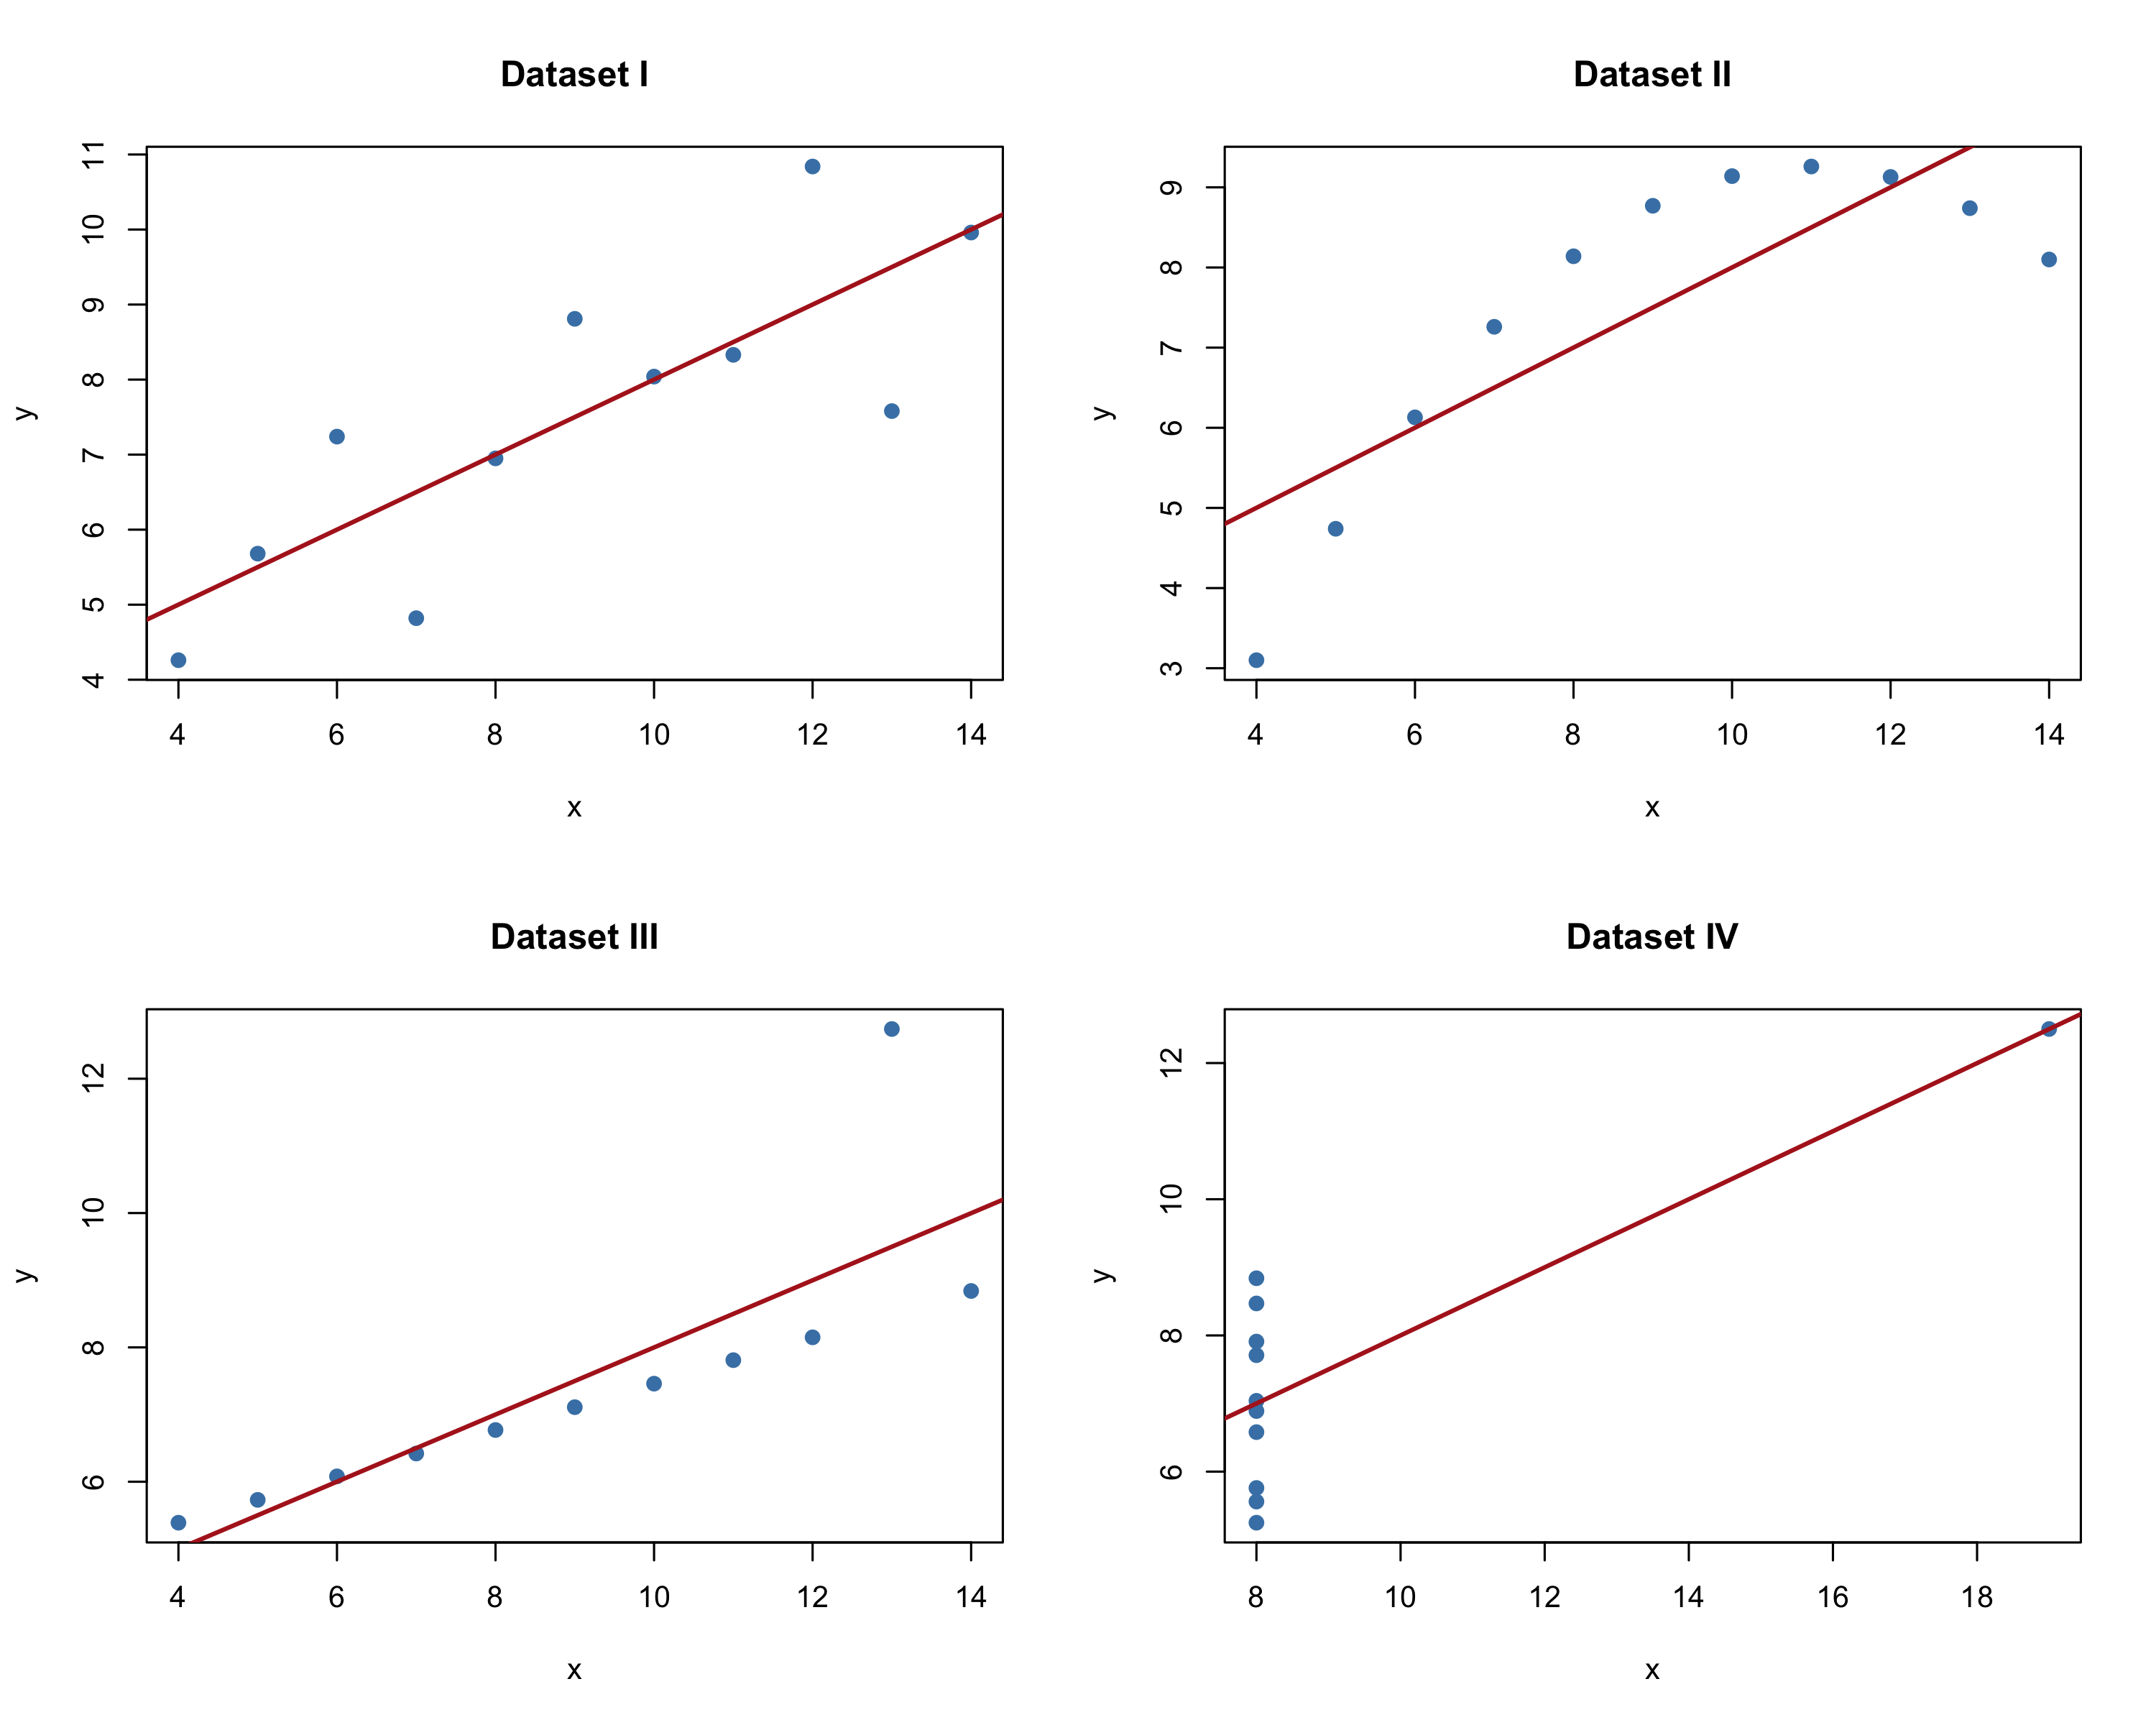
\includegraphics[width=0.85\textwidth]{scatterplots.png}

\caption{Scatterplots of \texttt{y} vs.\ \texttt{x} for each dataset,
with the fitted OLS line overlaid.}

\end{figure}

% ---------------------------------------------------------------------
\subsection{Improving the Trading Strategy (1.5)}
% ---------------------------------------------------------------------

\textit{For each stock, describe the \underline{one} improvement to your
trading strategy (relative to your answer in 1.3) that the scatterplot
suggests is most important.}

\noindent\textbf{Answer:}

Although the four stocks have nearly identical summary statistics and OLS estimates, their scatterplots reveal very different patterns in the relationship between $x$ and $y$. Therefore, the linear trading strategy we proposed in 1.3 should be adjusted separately for each stock based on the structure revealed by the scatterplots.

\vspace{1em}

\noindent\textbf{Dataset I:}

The data points are distributed roughly symmetrically around the fitted line. This suggests the linear relationship provides a reasonable description of the data. Therefore, I would retain the original strategy from 1.3: go long when $x$ is high and short when $x$ is low.

\vspace{1em}

\noindent\textbf{Dataset II:}

The scatterplot shows a clear nonlinear, inverted-U-shaped relationship of $y$ = a$x^2$+b. $y$ initially increases with $x$, but after reaching a peak, the relationship becomes negative. Therefore, I would use different trading rules on the two sides of the turning point: go long as $x$ rises before the peak, but reverse the strategy after the peak and short as $x$ rises further.

\vspace{1em}

\noindent\textbf{Dataset III:}

The scatterplot shows that there is one unusual observation that pulls the entire fitted line upward, making the positive relationship between $x$ and $y$ appear stronger than it is for most of the data. Therefore, I would lower my expectation to the marginal returns. I would still go long when $x$ is high and short when $x$ is low, but with smaller positions and less confidence in the signal.

\vspace{1em}

\noindent\textbf{Dataset IV:}

In this plot, for most observations, there is no clear relationship between $x$ and $y$. The apparent positive linear relationship is driven almost entirely by a single high-leverage observation.

Therefore, I would not rely on the fitted linear rule. And I would avoid taking long or short positions based on $x$ alone without additional evidence.

% =====================================================================
\section{Predicting house prices (40 points)}
% =====================================================================

\subsection{Data Preparation (2.1)}

The following code loads the Connecticut property data, first constructs the
true assessed value, then expresses both assessed value and sale amount in
\$1,000s. Eventually we filters the sample to single-family homes in New Haven
listed in 2008 with true assessed values below \$250,000.

\vspace{0.5em}

\begin{lstlisting}[style=rcode]
# ---- 2.1.1: Load the data ----
ct <- read.csv("ps1/ct_property_data.csv")

# ---- 2.1.2: Create assessedvalue_true ----
# Tax-assessed value in CT is 70% of true market value,
# so dividing by 0.7 recovers the true value.
ct$assessedvalue_true <- ct$assessedvalue / 0.7

# ---- 2.1.3: Express in $1,000s ----
ct$assessedvalue_true <- ct$assessedvalue_true / 1000
ct$saleamount <- ct$saleamount / 1000

# ---- 2.1.4: Filter ----
ct_filtered <- ct[
    ct$residentialtype == "Single Family" &
        ct$town == "New Haven" &
        ct$listyear == 2008 &
        ct$assessedvalue_true < 250,
]
\end{lstlisting}

\vspace{0.5em}

The resulting sample contains \textbf{279 observations}.

% ---------------------------------------------------------------------
\subsection{Manual Prediction Rule (2.2)}
% ---------------------------------------------------------------------

The manual prediction rule is:
\[
\text{Predicted sale amount} = 0.8 \times \text{true assessed value}.
\]

We chose a slope of 0.8 because the true assessed value represents the tax assessor's estimate of a house's market value, while the actual transaction price may be lower when housing-market conditions weaken. Because the observations are from 2008, during a time where major housing-market downturn, assessments may have adjusted more slowly than sale prices. We therefore use 80\% of the assessed value as a simple initial prediction.

The intercept is set to zero because the rule assumes that sale price changes in direct proportion to assessed value. This rule is based on economic reasoning rather than estimated from the 2008 sample, so the later residual and OLS analyses can show how it should be improved.

% ---------------------------------------------------------------------
\subsection{Residuals and Model Improvement (2.3)}
% ---------------------------------------------------------------------

A residual is calculated by deducting the estimated value from the actual value of sales. If the residual is positive, the house sells at a higher price than predicted manually. Otherwise, it sells for a lower price than was predicted.
\[
\text{Residual} = \text{actual sale amount} - \text{predicted sale amount}.
\]

\begin{figure}[h]
\centering
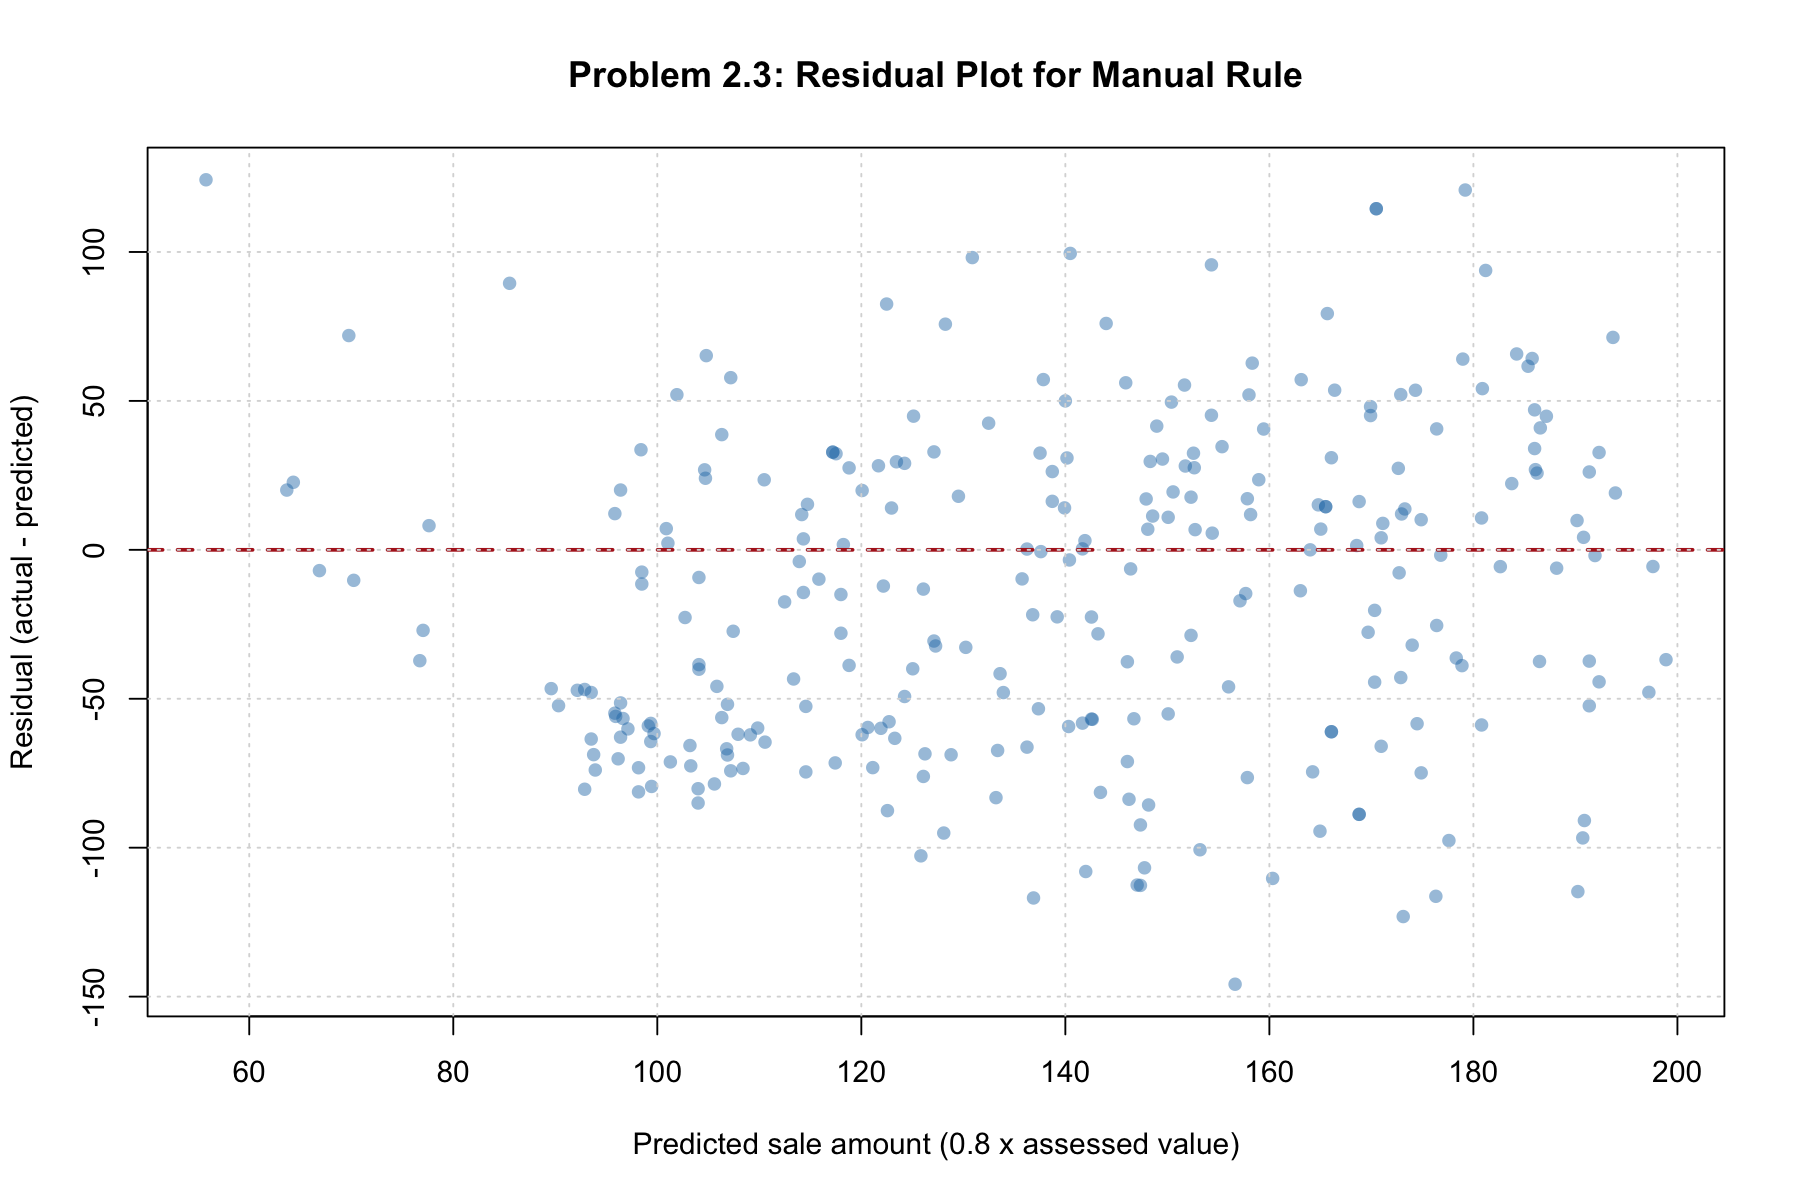
\includegraphics[width=0.75\textwidth]{person2/problem2_3_residual_plot.png}
\caption{Residuals from the manual prediction rule for the 2008 sample.}
\end{figure}

The residual plot exhibits an identifiable pattern, instead of being randomly distributed around zero. There are a lot of negative residuals among those houses which have lower to medium level of assessment value, meaning that the manual rule tends to overestimate their price. On the other hand, as the assessment value increases, the residuals are becoming increasingly positive, and hence the manual rule underestimates their prices.

In order to make the manual prediction rules better, my suggestion would be to decrease the intercept and increase the slope.

% ---------------------------------------------------------------------
\subsection{Manual OLS Estimates (2.4)}
% ---------------------------------------------------------------------

OLS slope is equal to the sample covariance between the assessed value and sales amount divided by the sample variance of the assessed value. The intercept will shift the line to pass through the means of the samples.
\[
\hat{\beta}_1 = \frac{\text{Cov}(x, y)}{\text{Var}(x)} \qquad \text{and} \qquad \hat{\beta}_0 = \bar{y} - \hat{\beta}_1 \bar{x}
\]

\begin{table}[h]
\centering
\caption{Manual OLS estimates from sample moments}
\begin{tabular}{lc}
\toprule
Quantity & Estimate \\
\midrule
Mean true assessed value & 173.767993 \\
Mean sale amount & 123.961767 \\
Covariance of $x$ and $y$ & 1{,}657.481376 \\
Variance of $x$ & 1{,}642.393594 \\
OLS intercept & -51.402538 \\
OLS slope & 1.009186 \\
\bottomrule
\end{tabular}
\end{table}

The resulting prediction rule is sale amount $= -51.402538 + 1.009186 \times$ assessed value. Relative to the manual rule, OLS uses a lower intercept and a steeper slope.

% ---------------------------------------------------------------------
\subsection{Numerical Optimization (2.5)}
% ---------------------------------------------------------------------

The numerical optimization was used to find the OLS estimates. The algorithm had a normal convergence and returned a code of 0. The coefficient values are within $4.01\times10^{-8}$ of the manually calculated OLS values.

\begin{lstlisting}[style=rcode]
sse <- function(parameters) {
  sum((y - parameters[1] - parameters[2] * x)^2)
}
optimization <- optim(par = c(0, 0.8), fn = sse, method = "BFGS")
\end{lstlisting}

\begin{table}[h]
\centering
\caption{Manual rule, manual OLS, and numerical OLS estimates}
\begin{tabular}{lccc}
\toprule
Method & Intercept & Slope & SSE \\
\midrule
Manual rule & 0.000000 & 0.800000 & 863{,}077.094 \\
Manual OLS & -51.402538 & 1.009186 & 779{,}881.121 \\
optim & -51.402539 & 1.009186 & 779{,}881.121 \\
\bottomrule
\end{tabular}
\end{table}

% ---------------------------------------------------------------------
\subsection{Manual and OLS Prediction Rules (2.6)}
% ---------------------------------------------------------------------

This scatter plot shows the two regression equations in comparison with the observed values of sale prices. The regression equation using OLS estimates gives the smallest squared error of predictions and reduces the SSE to 83,195.973 and RMSE from 55.619 to 52.869. The lines intersect at higher assessment values but diverge at lower values due to negative intercept.

\begin{figure}[h]
\centering
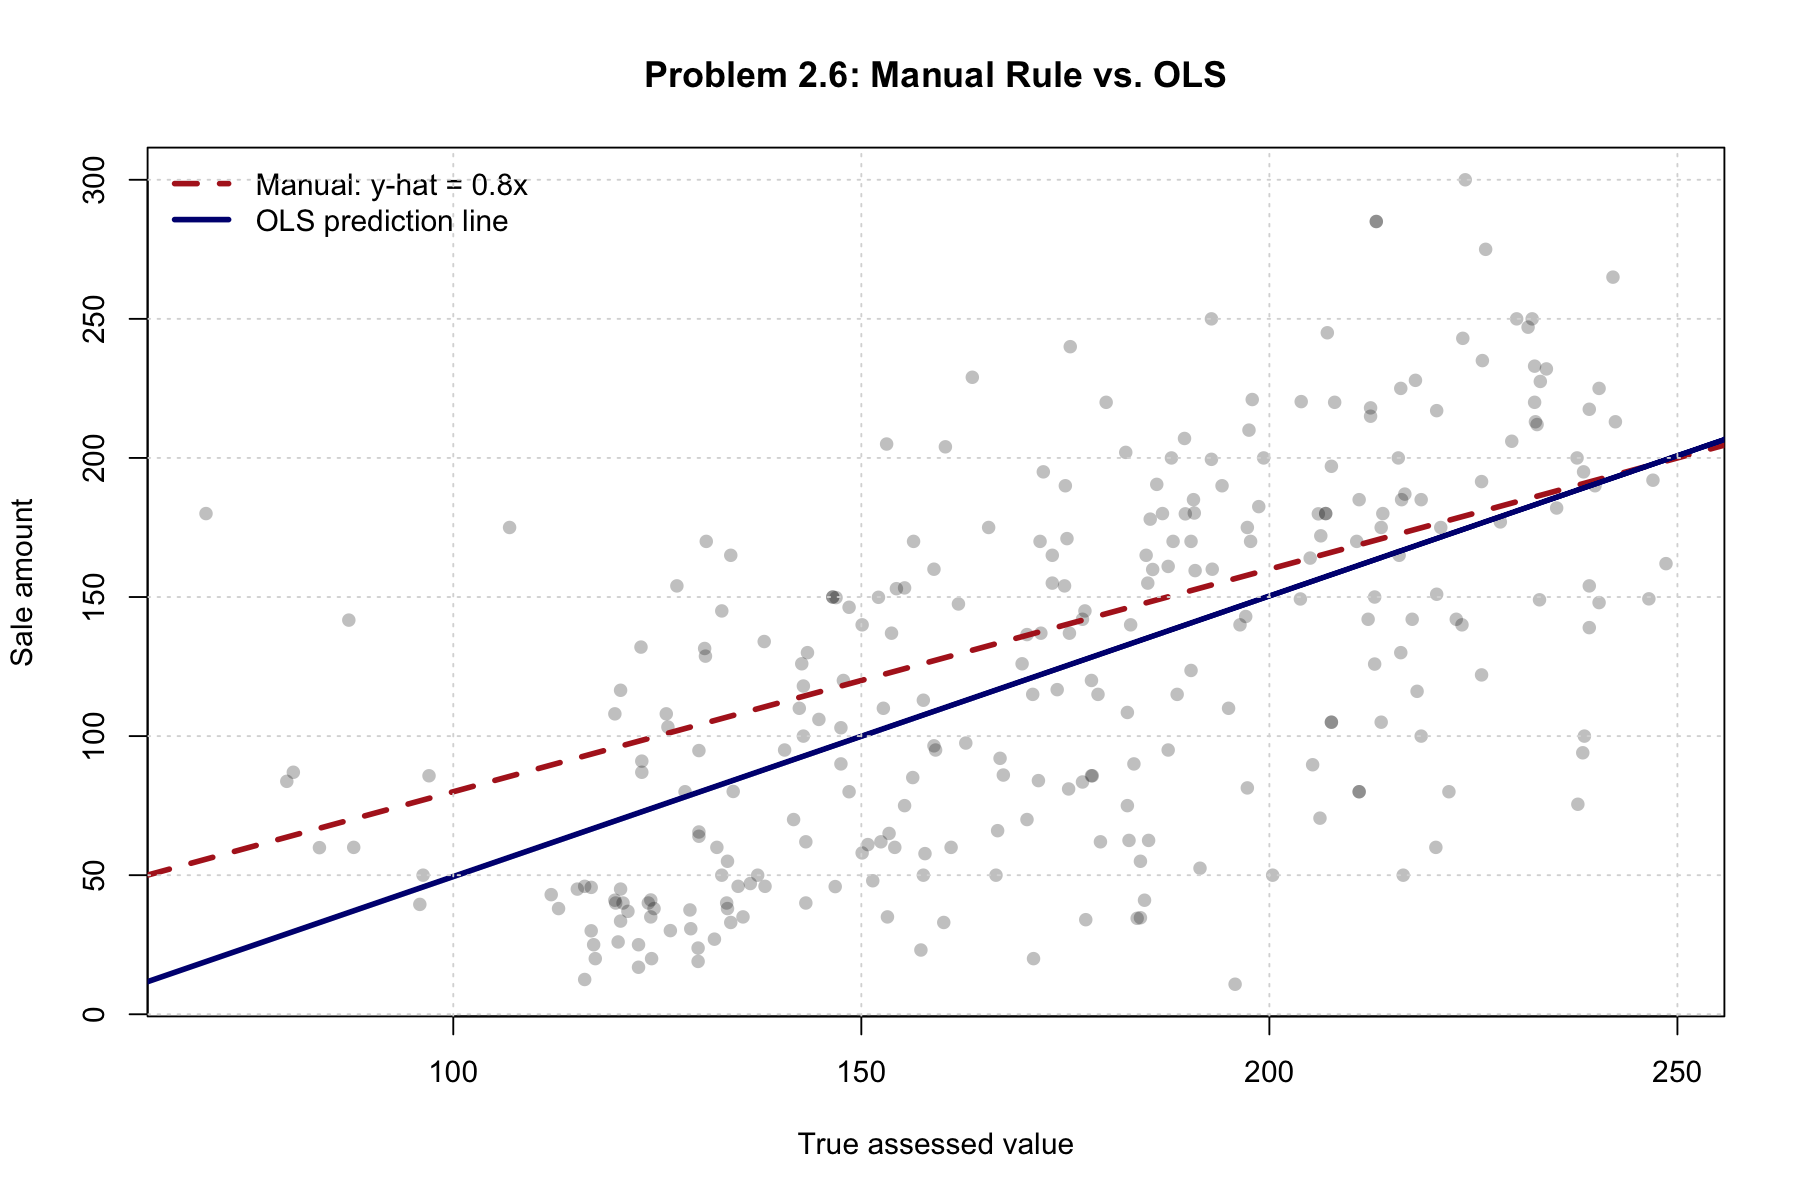
\includegraphics[width=0.75\textwidth]{person2/problem2_6_manual_vs_ols.png}
\caption{Sale amounts with the manual and 2008 OLS prediction lines.}
\end{figure}

% ---------------------------------------------------------------------
\subsection{Prediction Rule for 2023 (2.7)}
% ---------------------------------------------------------------------

Of the three options that we have, I will use the OLS class rule from 2020 for forecasting in 2023, which can be given by the equation Sale amount $= -4.69 + 1.37 \times$ Assessed Value. The sample from 2020 is more recent compared to 2023 and is less likely to be outdated than the 2008 OLS class rule or the manual rule. This is based on the assumption that the value of the assessed value was relatively stable from 2020 to 2023.

% ---------------------------------------------------------------------
\subsection{Annual OLS Estimates (2.8)}
% ---------------------------------------------------------------------

For this yearly sample, the same property, town, and assessed value limitations have been applied, however the limitation for 2008 has been discarded. The obtained sample is represented by 3,819 transactions within 14 years of listings, which occurred between 2007 and 2021. There are no observations related to 2016 year in the source file according to the sample definition criteria.

\begin{table}[h]
\centering
\caption{Annual OLS estimates, 2007--2021}
\begin{tabular}{lccc}
\toprule
Listing year & Observations & Intercept & Slope \\
\midrule
2007 & 316 & 5.697 & 0.900 \\
2008 & 279 & -51.403 & 1.009 \\
2009 & 289 & 2.984 & 0.728 \\
2010 & 167 & -69.866 & 1.091 \\
2011 & 224 & -8.620 & 0.990 \\
2012 & 250 & -22.542 & 1.025 \\
2013 & 233 & -31.225 & 1.128 \\
2014 & 248 & -19.699 & 1.009 \\
2015 & 264 & -26.429 & 1.095 \\
2017 & 277 & -17.426 & 1.114 \\
2018 & 262 & -21.175 & 1.156 \\
2019 & 317 & 11.804 & 1.048 \\
2020 & 381 & 20.877 & 1.216 \\
2021 & 312 & 29.437 & 1.136 \\
\bottomrule
\end{tabular}
\end{table}

\begin{figure}[h]
\centering
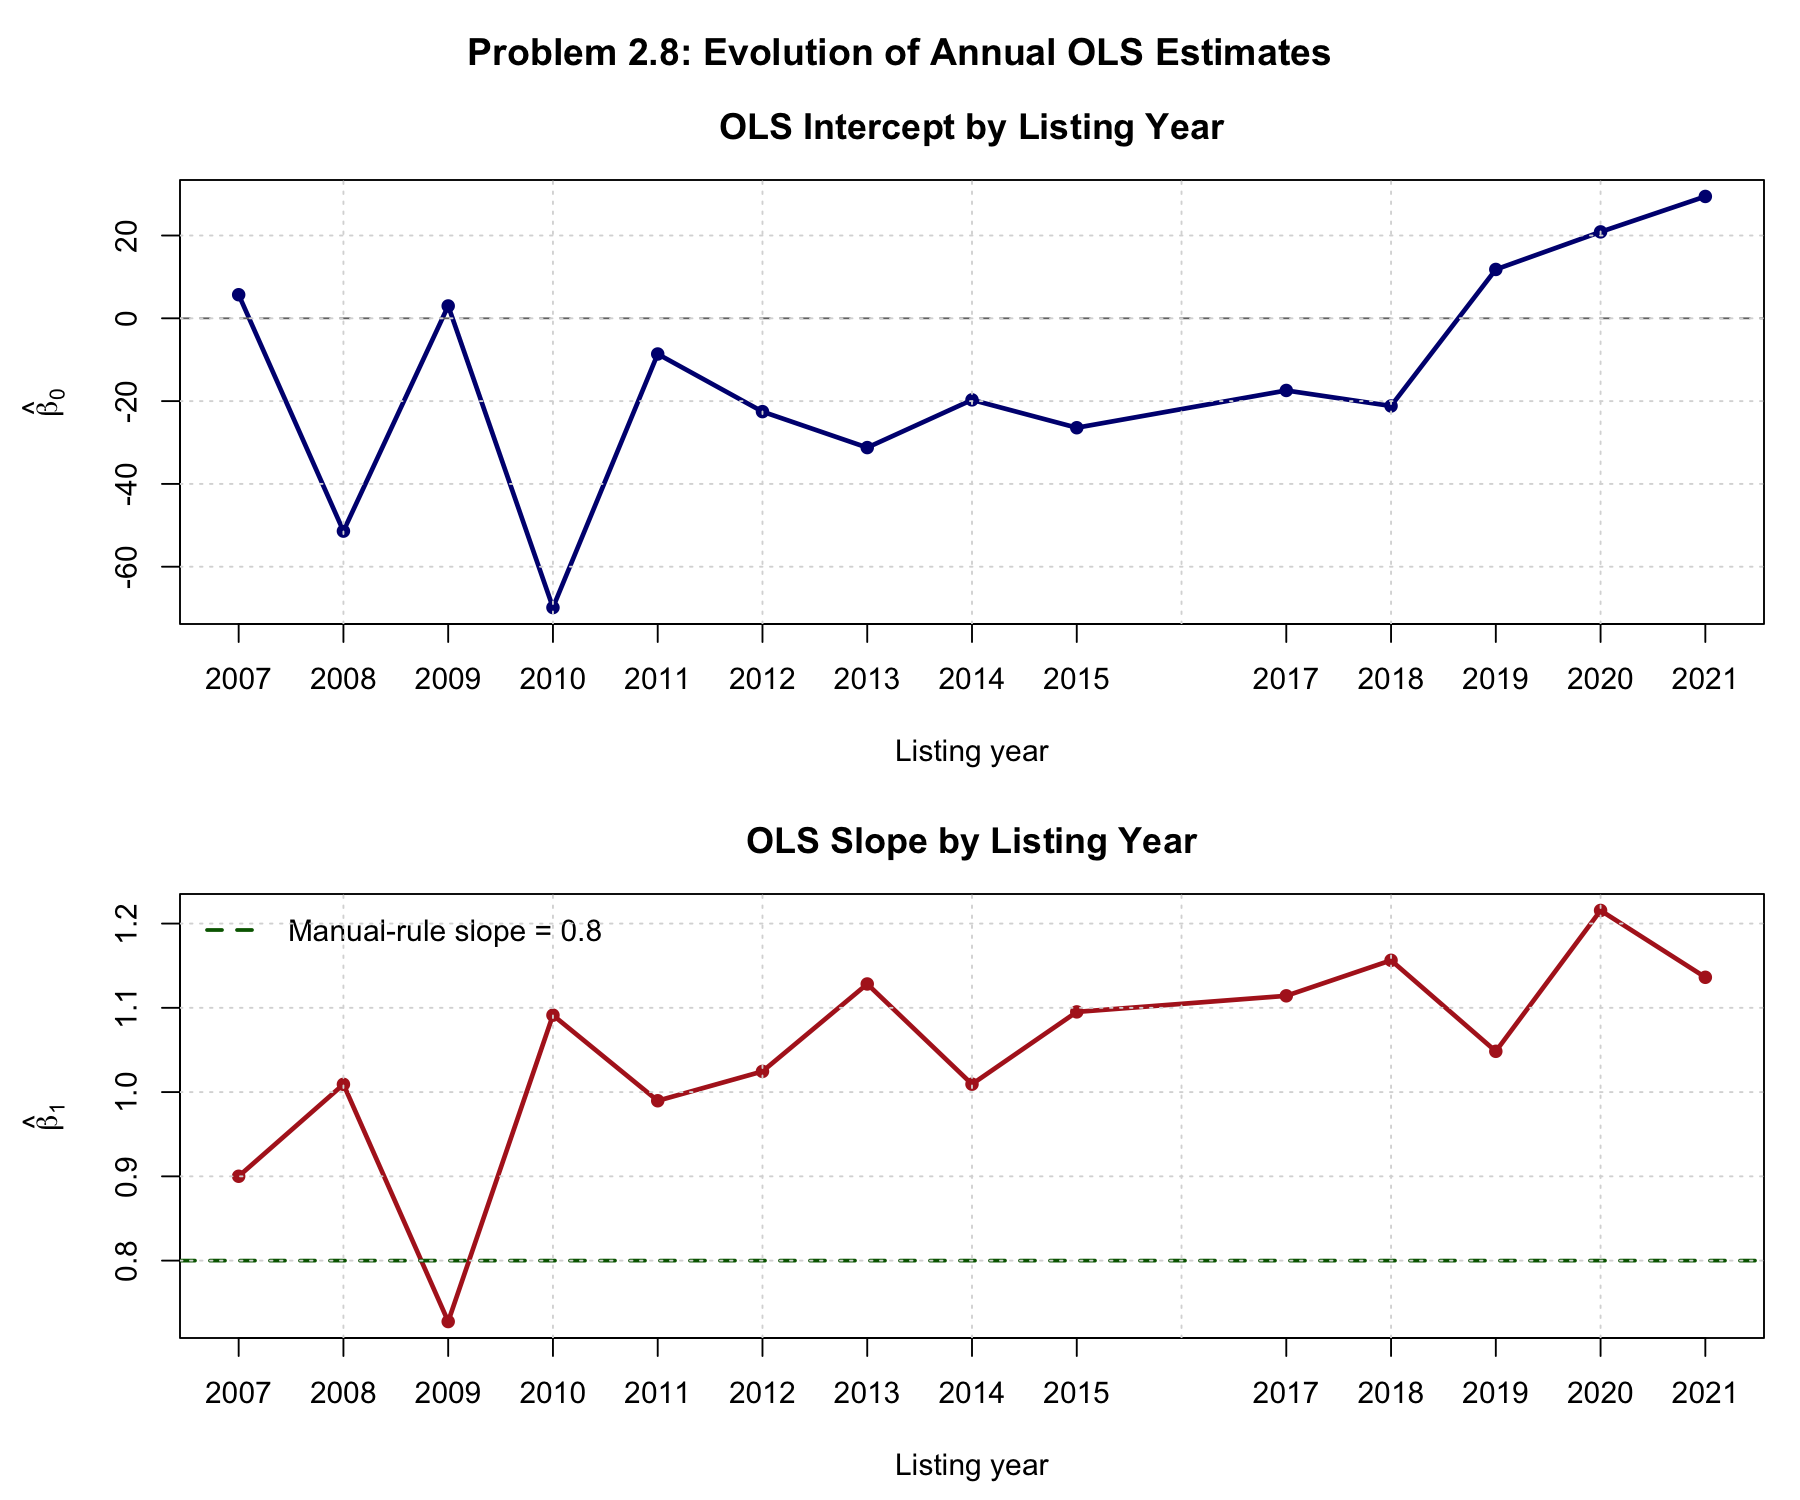
\includegraphics[width=0.75\textwidth]{person2/problem2_8_annual_ols_trends.png}
\caption{Annual OLS intercepts and slopes for the all-years sample.}
\end{figure}

Both variables are dynamic. The slope starts at 0.728 in 2009 and increases up to 1.216 in 2020, whereas the intercept decreases from -69.866 in 2010 to 29.437 in 2021. This indicates that the connection between the variables is dynamic and that there is no static pattern linking the values of assessed property and sale prices by year of listing.

\vspace{1em}
\noindent\textbf{Conclusion:} The 2008 OLS model is better than the manual model since it matches the data and reduces the total error sum. The numerical and equation OLS models give similar answers. The annual data show that the regression relationship varies with time, making the 2020 classroom model more sensible among the given models to predict 2023.

% =====================================================================
\section{Predicting portfolio risk (40 points)}
% =====================================================================

\subsection{Return Statistics (3.1--3.2)}

Table \ref{tab:returnstats} shows the sample means and standard deviations of monthly excess returns for the three long-short factors (Value, Momentum, Quality) and the market over the sample period.

\begin{table}[h]
\centering
\caption{Sample means and standard deviations of monthly excess returns}
\label{tab:returnstats}
\begin{tabular}{lcccc}
\toprule
 & Market & Value & Momentum & Quality \\
\midrule
Mean & 0.0069 & 0.0032 & 0.0033 & 0.0031 \\
SD & 0.0451 & 0.0393 & 0.0362 & 0.0164 \\
\bottomrule
\end{tabular}
\end{table}

\subsection{Correlation Matrix (3.3)}

Table \ref{tab:corrmatrix} reports the correlation matrix of the same four return series.

\begin{table}[h]
\centering
\caption{Correlation matrix of monthly excess returns}
\label{tab:corrmatrix}
\begin{tabular}{lcccc}
\toprule
 & Market & Value & Momentum & Quality \\
\midrule
Market & 1.00 & -0.27 & -0.34 & -0.18 \\
Value & -0.27 & 1.00 & -0.25 & -0.14 \\
Momentum & -0.34 & -0.25 & 1.00 & 0.23 \\
Quality & -0.18 & -0.14 & 0.23 & 1.00 \\
\bottomrule
\end{tabular}
\end{table}

All three factors (Value, Momentum, Quality) are negatively correlated with the market, consistent with them being long-short ``hedged'' strategies. Value and Momentum are negatively correlated ($-0.25$), Value and Quality are negatively correlated ($-0.14$), and Momentum and Quality are positively correlated ($0.23$), offering less diversification benefit as a pair.

\subsection{Portfolio Risk (3.4)}

The Portfolio allocates 50\% to Value, 25\% to Momentum, and 25\% to Quality. Using the general portfolio variance formula,
\[
\text{Var}(P) = \sum_i \sum_j w_i w_j \sigma_i \sigma_j \, \text{corr}(i,j), \qquad SD(P) = \sqrt{\text{Var}(P)},
\]
with the sample standard deviations and correlations in 3.1--3.3, the predicted standard deviation of The Portfolio is 1.97\% per month.

\subsection{Market Betas (3.5)}

Table \ref{tab:betas} reports the market beta estimates from separate OLS regressions of Value, Momentum, and Quality on the market return.

\begin{table}[h]
\centering
\caption{Market beta estimates}
\label{tab:betas}
\begin{tabular}{lccc}
\toprule
 & Value & Momentum & Quality \\
\midrule
Market beta & -0.2387 & -0.2747 & -0.0672 \\
\bottomrule
\end{tabular}
\end{table}

\subsection{Residual Variances (3.6)}

Table \ref{tab:residvar} reports the sample variance of the residuals from each of the three market regressions.

\begin{table}[h]
\centering
\caption{Residual variances}
\label{tab:residvar}
\begin{tabular}{lccc}
\toprule
 & Value & Momentum & Quality \\
\midrule
Residual variance & 0.001425 & 0.001155 & 0.000261 \\
\bottomrule
\end{tabular}
\end{table}

\subsection{Portfolio Risk Using the Market Model (3.7)}

The Portfolio allocates 50\% to Value, 25\% to Momentum, and 25\% to Quality. Using the market-model variance formula,
\[
\text{Var}(P) = \beta_P^2 \, \text{Var}(\text{Market}) + w_V^2 \, \text{Var}(e_V) + w_M^2 \, \text{Var}(e_M) + w_Q^2 \, \text{Var}(e_Q)
\]
where $\beta_P = -0.2048$, the predicted standard deviation of The Portfolio is 2.30\% per month.

\subsection{Why Are the Two Risk Predictions Different? (3.8)}

The sample-covariance approach in 3.4 gives a portfolio standard deviation of 1.97\%, while the market-model approach in 3.7 gives 2.30\%. The estimates differ because 3.4 uses the observed covariances among the three factors, whereas 3.7 attributes common risk to the market and treats the remaining residual risks as uncorrelated.

\subsection{Preferred Risk Prediction (3.9)}

I prefer the estimate from 3.4 because it uses the observed covariance structure directly. Since the regression residuals remain correlated, the market-model assumptions in 3.7 do not fully capture the relationships among the three factors.

\end{document}
